Our simple DHT has a predefined number of extents (e.g. files) to which it can write and a predefined amount of initial nodes. Each key of the initial nodes is hashed with SHA-1 and mapped to an identifier circle and that will be the node's id. In our simple example we start with a fixed number of nodes so we can construct the Chord ring easily by sorting the nodes by their ids. With sorted nodes we can use a greater or equal variation of binary search (that wraps) to construct the finger tables and predecessor links for the nodes.

After creating the nodes we add the predefined extents in a similar manner. Each key is hashed and mapped to the identifier circle and added to its successor node using binary search. For each extent, $N$ number of copies is created and distributed to the next $N$ nodes on the Chord ring. This approach has the downside of putting the entire load of a failing node on its neighbor although nodes in our simplified version will neither fail or leave.

Only two operations are supported when the DHT has been initialized, writing to an extent and adding a new node. Given a requesting node and an extent to write to, we start from said node and look for the extent's successor using the finger tables to jump as far ahead as we can, not succeeding the id on the Chord ring. This will guarantee logarithmic jumps in order to find a successor. When found we update the extent and all of its copies.

Adding new nodes was by far the most challenging part of our implementation. We do keep track of sorted node ids for statistical and unit testing purposes but using them to find nodes would defeat the purpose of a distributed system. As before, we start by hashing the node's key but now we use the finger tables to find its successor. The new node is stored and we update the predecessor and successor links for the new node and the two adjacent nodes and construct a finger table for the new node (using the finger tables already in place). Instead of stabilizing the finger tables of the remaining nodes in a background task we do so right away and finally we move the extents that should now belong to the new node as well as moving the copies so the $N$ successors system persists as shown in Figure \ref{fig:extentmove}.

\begin{figure}[ht!]
    \centering
    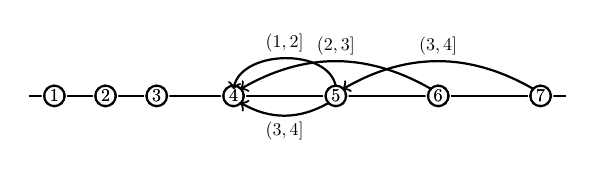
\begin{tikzpicture}[thick,scale=0.65, every node/.style={scale=0.65}]
\draw (0,0) -- (10.5,0);
\foreach \x [count=\xi] in {0.5, 1.5, 2.5, 4, 6, 8, 10} {
    \fill[white] (\x,0) circle (0.25);
    \ifthenelse{\xi = 4}
    {\draw[dotted] (\x,0) circle (0.2) node {$\xi$};}
    {\draw (\x,0) circle (0.2) node {$\xi$};}
}
\def\offset{0.13}
\draw [->] (10-\offset,0+\offset) to [out=150,in=30] node[midway, above] {$(3,4]$} (6+\offset,0+\offset);
\draw [->] (8-\offset,0+\offset) to [out=150,in=30] node[midway, above] {$(2,3]$} (4+\offset,0+\offset);
\draw [->] (6,0+\offset+.05) to [out=100,in=80] node[midway, above] {$(1,2]$} (4,0+\offset);
\draw [->] (6-\offset,0-\offset) to [out=-150,in=-30] node[midway, below] {$(3,4]$} (4+\offset,0-\offset);
\end{tikzpicture}
    \caption{Movement of extents and copies ($N=2$) when a node is added (4) with copies above and original extents below. Intervals are node label range of extent successors.}
    \label{fig:extentmove}
\end{figure}